%%%%%%%%%%%%%%%%%%%%%%%%%%%%%%%%%%%%%%%%%%%%%%%%%%%%%%%%%%%%%%%%%%%%%%%%%%%%%%%%%%%%%%%%%%%%%%%%%
%% Funktionen                                   
%%%%%%%%%%%%%%%%%%%%%%%%%%%%%%%%%%%%%%%%%%%%%%%%%%%%%%%%%%%%%%%%%%%%%%%%%%%%%%%%%%%%%%%%%%%%%%%%%
\begin{flushleft}
	\section{Funktionen\formelbuchred{48}}
		\subsection{Einleitung}
			\begin{minipage}[t]{5cm}
				\textbf{Schreibweisen:}\\
				$f:D_f \rightarrow W_f$ mit $x \mapsto f(x)$\\
				$f:x \mapsto f(x)$ mit $x \in D_f$\\
				$y=f(x)$ mit $x \in D_f$
			\end{minipage}
			\hfill
			\begin{minipage}[t]{8cm}
				\textbf{Definitionen:}\\
				$x \Rightarrow$ Argument oder Variable von $f$\\
				$f(x) \Rightarrow$ Funktionswert, Wert von $f$ an der Stelle $x$\\ 
				$x \mapsto f(x)$ oder $y=f(x) \Rightarrow$ Zuordnungsvorschrift\\
				$D_f \Rightarrow$ Definitonsmenge oder Definitionsbereich\\ 
				$W_f \Rightarrow$ Wertemenge oder Wertebereich
			\end{minipage}
			\hfill
			\begin{minipage}[t]{4cm}
				\textbf{Achsenbezeichnungen:}\\
				Abszisse = X-Achse\\
				Ordinate = Y-Achse\\
				Applikate = Z-Achse
			\end{minipage}	

		\subsection{Transformationen}
			\begin{minipage}[c]{5cm}
				$\mathbf{\pm \; {\color{red}a} \cdot f( \; \pm \; {\color{blue}b}x \; \pm \; 
				{ \; \color{green}c}) \; \pm \; {\color{cyan}d}}$\\
				 1.schieben 2.stecken\\
				$ $\\
				$\mathbf{\pm \; {\color{red}a} \cdot f( \; \pm \; {\color{blue}b} ( x \; \pm
				{ \; \color{green}c})) \; \pm \; {\color{cyan}d}}$\\
				1.strecken 2.schieben\\	
			\end{minipage}
			\begin{minipage}[t]{10cm}
				\begin{tabular}{lll}
					1. &\textbf{{\color{red}a}} &Vertikale (y-Richtung) Streckung um \textbf{a} bzw. Spiegelung an x bei \textbf{-a}\\
					2. &\textbf{{\color{blue}b}} &Horizontale (x-Richtung) Streckung um \textbf{1/b} bzw. Spiegelung an y bei \textbf{-b}\\
					3. &\textbf{{\color{green}c}} &Verschiebung nach links (\textbf{+c}) oder rechts (\textbf{-c}) (vertikale Verschiebung)\\
					4. &\textbf{{\color{cyan}d}} &Verschiebung nach oben (\textbf{+d}) oder unten (\textbf{-d}) (horizontale Verschiebung)
				\end{tabular}
			\end{minipage}
				
			\subsubsection{Spiegelung}
				an X-Achse: Polarit"at von $f$ "andern\\
				an Y-Achse: Polarit"at von $x$ "andern\\
			
		\subsection{Spezielle Funktionen}
			\begin{minipage}[t]{6cm}
				\textbf{Identit"at:}\\
				Schreibweise: $f(x)=x$\\\\
				Definition:\\
				Der X-Wert ist gleich dem Y-Wert
			\end{minipage}
			\hfill
			\begin{minipage}[t]{6cm}
				\textbf{Signumfunktion:}\\
				Schreibweise: $f(x)=sgn(x)$\\
				Definiton: $y=\left\{\begin{array}{l}\text{1, falls $x>0$}\\
				\text{0, falls $x=0$}\\\text{-1, falls $x<0$}\end{array}\right.$
			\end{minipage}	
			\hfill
			\begin{minipage}[t]{6cm}
				\textbf{Gauss-Klammer (floor):}\\
				Schreibweise: $f(x)=\left[x\right]$\\\\
				Definition:\\
				rundet den Y-Wert ganzzahlig ab
			\end{minipage}
				
		\subsection{Umkehrfunktion\formelbuchred{52}}
		\begin{tabbing}
			-----------------------------\= \kill
			Schreibweise: $f^{-1}$ \> Definition: ein Y-Wert darf nur einmal vorkommen und $W_f$ muss $\in D_f$ sein\\
			Ist eine Funktion $f$ auf einem Intervall $D$ streng monoton, dann existiert f"ur dieses Intervall die Umkehrfunktion $f^{-1}$
		\end{tabbing}
		
		\subsection{Verkettung oder mittelbare Funktion}
		\begin{tabbing}
			--------------------\=----------------------------------------------\=------------------\=-----------------\=----------------------\= \kill	
			Schreibweise: \> $h(x)=g \circ f \Rightarrow h(x)=g(f(x))$ \> Sprechweise: \> \textit{g nach f} \> Wertebereiche: \> $W_h=W_g \rightarrow D_h=D_f$\\
								    \> $h(x)=f \circ g \Rightarrow h(x)=f(g(x))$ \>  \> \textit{f nach g} \> \> $W_h=W_f \rightarrow D_h=D_g$
		\end{tabbing}
		
	 		\textbf{Wichtig:} Funktionen sind nacheinander ausf"uhrbar, wenn der $W_f \subset D_g$ bzw. $W_g \subset D_f$  ist.
			
		\subsection{Beschr"anktheit\formelbuchred{51}}
			
		\subsection{Monotonie\formelbuchred{50}}
			\begin{tabbing}
				-------------------------------------------------------------------------\= \kill
				\textbf{monoton wachsend} $\longrightarrow x_1<x_2 \Rightarrow f(x_1)\leq f(x_2)$\>
				\textbf{streng monoton wachsend} $\longrightarrow x_1<x_2 \Rightarrow f(x_1) < f(x_2)$\\
				\textbf{monoton fallend} $\longrightarrow x_1<x_2 \Rightarrow f(x_1)\geq f(x_2)$\>
				\textbf{streng monoton fallend} $\longrightarrow x_1<x_2 \Rightarrow f(x_1)>f(x_2)$
			\end{tabbing}		
\newpage
		\subsection{Gerade/Ungerade Funktionen\formelbuchred{51}}
			Funktion ist \textbf{gerade} wenn $f(-x)=f(x)\Rightarrow$ Achsensymmetrisch\\
			Funktion ist \textbf{ungerade} wenn $ f(-x)=-f(x)\Rightarrow \text{Punktsymmetrisch}$\\
			Funktion ist \textbf{periodisch} wenn $f(x) = f(x \pm p)\Rightarrow \text{wiederholt sich im Abstand p}$ \qquad
			$\text{f"ur beide gilt: } \underbrace{ x \in D_f \land -x \in D_f}_{D_f \text{ ist } \textbf{symmetrisch}}$\\
			\textbf{Wichtig:} Um zu beweisen das eine Funktion gerade bzw. ungerade ist, zeigt man indem man beweist, dass es f"ur \underline{einen} Punkt \underline{nicht} stimmt!\\
		
		\subsection{Ganzrationale Funktionen (Polynom)\formelbuchred{62,64}}
			Aussehen: \[f(x)=a_nx^{n}+a_{n-1}x^{n-1}+\cdots+a_1x+a_0\]\\
			Nullstellen bestimmen:\\
			\begin{itemize}
				\item falls Polynom ($ax^{2}+bx+c$) quadratische L"osungsformel: $\frac{-b\pm\sqrt{b^{2}-4ac}}{2a}$
				\item faktorisieren mit Hilfe von Binomen
				\item faktorisieren mit Hilfe des \textbf{Hornerschemas\formelbuchred{957}}
			\end{itemize}
			\textbf{Wichtig:} eine ganzrationale Funktion $n$-ten Grades hat h"ochstens $n$ verschiedene Nullstellen

		\subsection{Hornerschema\formelbuchred{965}}
			\begin{minipage}[t]{9cm}
				- Pfeile $\Rightarrow$ Multiplikation\\
				- Zahlen pro Spalte werden addiert\\
				\includegraphics[width=6cm]{./bilder/hornerschema_1.png}	\\
				$x_1 \Rightarrow$ Nullstelle (muss erraten werden, durch \textbf{ausprobieren}!!)\\
				oberste Zeile = zu zerlegendes Polynom			
			\end{minipage}
			\begin{minipage}[t]{9cm}
				\textbf{Beispiel:}\\
				$f(x) = x^3-67x-126$\\
				\includegraphics[width=6cm]{./bilder/hornerschema_2.png}\\
				$\Rightarrow f(x) = (x-x_1)(b_2x^2 + b_1x + b_0) = (x+2)(x^2-2x-63)$	
			\end{minipage}
			Ergebnis der Form: $f(x)=(x-x_1)(g(x)+f(x_1)\hspace*{1cm}$ Linearfaktor: $(x-x_1)\hspace*{1cm}$ Polynom vom Grad $n-1$: $g(x)$ \\
		
		\subsection{Gebrochenrationale Funktionen\formelbuchred{62,66}}
			Aussehen: \[f(x)=\frac{p_m(x)}{q_n(x)}=\frac{a_mx^{m}+a_{m-1}x^{m-1}+\cdots+a_1x+a_0}{a_nx^{n}+a_{n-1}x^{n-1}+\cdots+a_1x+a_0}\]\\
			Definitionen:\\
			\begin{itemize}
				\item wenn $m<n$ ist $f$ \textbf{echt gebrochen}, wenn $m\geq n$ ist $f$ \textbf{unecht gebrochen}\\
				\item $x_1$ ist \textbf{Nullstelle} von $f$ falls $p_m(x_1)=0$ und $q_n(x_1)\neq0$ gilt $\rightarrow$ k-fache Nullstelle\\
				\item $x_1$ heisst \textbf{Polstelle} von $f$ falls $q_n(x_1)=0$ und $p_m(x_1)\neq0$ gilt $\rightarrow$ k-fache Polstelle\\
				\item $x_1$ heisst \textbf{L"ucke} von $f$ falls $q_n(x_1)=0$ und $p_m(x_1)=0$ gilt.\\
				\item Jede unecht gebrochene rationale Funktion l"asst sich als Summe einer ganzrationalen Funktion und einer echt gebrochenen Funktion
							schreiben. Dies ist m"oglich mit der \textbf{Polynomdivision\formelbuchred{15}}
			\end{itemize}			
			
		\subsection{Partialbruchzerlegung\formelbuchred{15}}
			\[f(x)=\frac{x^2+20x+149}{x^3+4x^2-11x-30} \Rightarrow \; \begin{array}{l}\text{Nenner faktorisieren mit}\\
			\text{Hornerschema\formelbuchred{965}, Binom}\end{array} \Rightarrow x^{3}+4x^{2}-11x-30=(x+2)(x^{2}+2x-15)=(8x+2)(x+5)(x-3)\]
			Ansatz:
			\[f(x)=\frac{x^2+20x+149}{x^3+4x^2-11x-30}=\frac{A}{x-3} + \frac{B}{x+2} + \frac{C}{x+5}=
			\frac{A(x+2)(x+5)+B(x-3)(x+5)+C(x-3)(x+2)}{(x-3)(x+2)(x+5)}\]
			Gleichungssystem \textbf{(Z"ahler gleichsetzen)} aufstellen mit beliebigen $x_i$-Werten (am Besten Polstellen oder 0,1,-1 w"ahlen):
			\[\begin{array}{l}x_1=3:\;-9+60+149=A\cdot5\cdot8\;\;\;\Rightarrow A=5\\
			x_2=-2:\;-4-40+149=B(-5)\cdot3\; \Rightarrow B=-7\\
			x_3=-5:\;-25-100+149=C(-8)(-3) \Rightarrow C=1 \end{array} \Rightarrow f(x)=\frac{5}{x-3}+\frac{7}{x+2}\frac{1}{x+5}\]
			weitere Ans"atze f"ur andere Typen von Termen: (Mehrere Werte f"ur $x$ verwenden, auch wenn kein Koeffizient 0 wird.)
			\[f(x)=\frac{5x^2-37x+54}{x^3-6x^2+9x}=\frac{A}{x}+\frac{B}{x-3}+\frac{C}{(x-3)^2}=\frac{A(x-3)^2+Bx(x-3)+Cx}{x(x-3)^2}\]
			\[f(x)=\frac{1,5x}{x^3-6x^2+12x-8}=\frac{A}{x-2}+\frac{B}{(x-2)^2}+\frac{C}{(x-2)^3}=\frac{A(x-2)^2+B(x-2)+C}{(x-2)^3}\]
			\[f(x)=\frac{x^2-1}{x^3+2x^2-2x-12}=\frac{A}{x-2}+\frac{Bx+C}{x^2+4x+6}=\frac{A(x^2+4x+6)+(Bx+C)(x-2)}{(x-2)(x^2+4x+6)}\]
							
		\subsection{Trigonometrische Funktionen\formelbuchred{76ff} Arcus\formelbuchred{86}}
			\begin{tabbing}
				-----------------------------------------------------------------\= \kill
				$\sin: D_f=[-\frac{\pi}{2},\frac{\pi}{2}]\rightarrow W_f=[-1,1]$ \> $\arcsin: D_f=[-1,1]\rightarrow W_f=[-\frac{\pi}{2},\frac{\pi}{2}]$\\
				$\cos: D_f=[0,\pi]\rightarrow W_f=[-1,1]$ \> $\arccos: D_f=[-1,1]\rightarrow W_f=[0,\pi]$\\
				$\tan: D_f=(-\frac{\pi}{2},\frac{\pi}{2})\rightarrow W_f=\mathbb{R}$ \> $\arctan: D_f=\mathbb{R}\rightarrow W_f=(-\frac{\pi}{2},\frac{\pi}{2})$\\
				$\cot: D_f=(0,\pi)\rightarrow W_f=\mathbb{R}$ \> arccot: $D_f=[-1,1]\rightarrow W_f=(0,\pi)$\\											
				Orthogonalit"atsbedingung: $m_1 \cdot m_2 = -1$
			\end{tabbing}


		\subsection{Schwingungen\formelbuchred{83}}

		\subsection{Potenz- und Wurzelfunktionen\formelbuchred{8,71}}
			\textbf{gerade Potenzfunktion:} $D_f=\mathbb{R} \rightarrow W_f=\mathbb{R}^+_0\;\;$
			\textbf{ungerade Potenzfunktion:} $D_f=\mathbb{R} \rightarrow W_f=\mathbb{R}$\\		
			\textbf{gerade Wurzelfunktion:} $D_f=\mathbb{R}^+ \rightarrow W_f=\mathbb{R}\;\;$
			\textbf{ungerade Wurzelfunktion:} $D_f=\mathbb{R} \rightarrow W_f=\mathbb{R}$
		
		\subsection{Hyperbolische Funktionen\formelbuchred{88} Areahyperbolicus\formelbuchred{92}}
			$	\sinh(x)=\frac{e^x-e^{-x}}{2}; D=\mathbb{R}, W=\mathbb{R} $
			\hspace{1.2cm}
			$ \cosh(x)=\frac{e^x+e^{-x}}{2}; D=\mathbb{R}, W=[1,\infty ) $
			\hspace{1.2cm}
			$ \tanh(x)=\frac{e^x-e^{-x}}{e^x+e^{-x}}; D=\mathbb{R}, W=(-1,1)  $
		
		\subsection{Logarithmus- und e-Funktion\formelbuchred{9,72}}
			\begin{minipage}[c]{9cm}
				\textbf{e-Funktion:} 
				$D_f=\mathbb{R} \rightarrow W_f=\mathbb{R}^+$ \\ \\
				%%$$e^x=\lim_{n \to \infty} (1+\frac{x}{n})^n$$				
				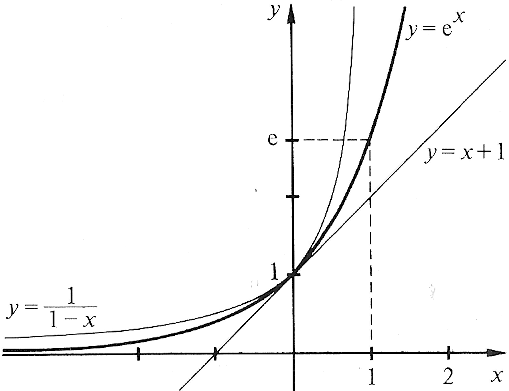
\includegraphics[height=4cm]{./bilder/funktionen_e.png} \\ \\
				$e^x \geq 1+x$ f"ur $x \in \mathbb{R}$\\
				$e^x \leq \frac{1}{1+x}$ f"ur $x < 1$\\
				$e=\lim\limits_{n\rightarrow\infty}(1+\frac{1}{n})^n$\\
			\end{minipage}
			\begin{minipage}[c]{9cm}
				\textbf{Logartihmus-Funktion:} $D_f=\mathbb{R}^+ \rightarrow W_f=\mathbb{R}$ \\ \\
				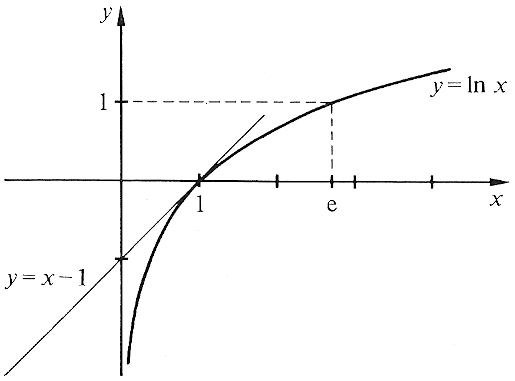
\includegraphics[height=4cm]{./bilder/funktionen_ln.png}\\
				$1-\frac{1}{x} \leq ln(x) \leq x-1$
			\end{minipage}
	
		\subsection{$\varepsilon - M$ - Kriterium\formelbuchred{53}}
			$|f(x) - g| < \varepsilon$ f"ur alle $x \geq M(\varepsilon)$

		\subsection{$\varepsilon - \delta$ - Kriterium\formelbuchred{53}}
			$|f(x) - g| < \varepsilon \qquad 0 < |x - x_0| < \delta(\varepsilon) \qquad \text{f"ur } x \rightarrow x_0$
	
		\subsection{K-Kriterium\formelbuchred{54}}
			$f(x) > K$ f"ur $x > M$, $K \in \mathbb{R}$\\
			$f(x) < k$ f"ur $x < m$, $ k \in \mathbb{R}$

\end{flushleft}
